\documentclass{article}
% NeurIPS style linked by course staff (neurips.cc/Conferences/2015/PaperInformation/StyleFiles).
\IfFileExists{nips15submit_e.sty}{%
  \usepackage{nips15submit_e,times}\nipsfinalcopy}{%
  \usepackage[text={5.5in,9in},centering]{geometry}\usepackage{times}}
\usepackage[T1]{fontenc}
\usepackage[utf8]{inputenc}
\usepackage{amsmath,amssymb,booktabs,graphicx,array}
\usepackage{tikz}
\usetikzlibrary{positioning,arrows.meta}
\usepackage[hidelinks]{hyperref}
\usepackage{url}

\title{In-Context Learning of Hidden Physical Dynamics\\from Push Interactions}
\author{Soomi Lee \quad Catherine Zhuang \quad Kenneth Llontop \quad David Jo\\
CS 182/282A Final Project, Report V1 (draft for peer review)\\
Code: \url{https://github.com/davidj24/cs182-final-project/tree/v1-report}}

\newcommand{\inprog}[1]{\textbf{[In progress]}~#1}

\begin{document}
\maketitle

\begin{abstract}
We ask whether a transformer that predicts how far a pushed block slides uses the \emph{information} in its push history about the hidden mass $m$ and friction $\mu$, or merely benefits from a longer context. We train a 9.5M-parameter causal transformer from scratch on an idealized 1D Coulomb-friction simulator and compare it with a Bayes estimator that knows the physics and the training prior. In a one-seed, noise-free pilot, one context push lowers median relative error from 56.3\% to 0.57\% (Bayes: 0.46\%). From two pushes on, the transformer stays between 0.33\% and 0.44\%, while Bayes falls below $10^{-4}\%$. Pushes at different forces help Bayes by many orders of magnitude on a new-force query; the transformer shows a matching advantage at two context pushes, but at four the answer changes with the checkpoint, so we call it inconclusive. On heavier cubes, context still helps, but relative error is about seven times larger.
\end{abstract}

\section{Introduction}
A robot that pushes an object cannot read its mass or friction from its appearance, yet both determine where the object ends up. Earlier pushes on the same object carry this information. \emph{In-context learning} (ICL) is a model's ability to use examples in its input to solve a new instance of a task with no weight update~\cite{brown2020}. A transformer trained across many objects could therefore adapt to a new one just by reading its push history.

A falling error-versus-context curve does not show \emph{why} the model improves. A longer history may contain more information about the hidden parameters, or it may only contain more tokens. Our pushing task separates the two. As Section~\ref{sec:physics} shows, in the ideal model repeating one force with different durations adds tokens but no new constraint on $(m,\mu)$ after the first push, whereas a second, different force identifies both parameters.

\textbf{Research question.} How do the number and type of pushes in a transformer's context determine how accurately it predicts a new push on an unseen cube, compared with an estimator that uses the same context optimally?

\textbf{Hypotheses} (from our proposal). \textbf{H1}: the transformer approaches the optimal estimator once the context size reaches the number of unknowns, $c=2$. \textbf{H2}: it needs pushes that differ in \emph{force}; pushes differing only in duration add no new information. \textbf{H3}: redundant pushes do not hurt, and under measurement noise repeated pushes help. \textbf{H4}: these patterns persist outside the training range.

\textbf{What this draft contains.} A pilot with one trained model that tests H1, H2, the noise-free part of H3 and one direction of H4. H1 is not supported at the precision the reference reaches. H2 is partly supported by the reference but unresolved for the transformer. Multiple seeds and measurement noise are still in progress (Section~\ref{sec:progress}).

\textbf{Changes since the proposal.} (i) The planned free-cube MuJoCo~\cite{todorov2012} contact scene failed our validation and was replaced by an idealized 1D sliding block (Appendix~\ref{app:contact}). All claims are about those ideal dynamics, not realistic contact. (ii) The pilot uses 1,000 training cubes, not about 10,000. (iii) It has one training seed and no noise. (iv) We use our own compact PyTorch implementation of a GPT-2-style model rather than the code of Garg et al.

\section{Related work}
\subsection{In-context learning of known function classes}
Brown et al.~\cite{brown2020} showed that a large language model can perform many tasks from a few demonstrations in its prompt, with no gradient updates. Because natural-language tasks have no known optimal answer, Garg et al.~\cite{garg2022} proposed a controlled testbed: train a small transformer from scratch on sequences $(x_1,f(x_1),x_2,f(x_2),\dots)$ with $f$ drawn from a function class, then test on unseen $f$. For linear functions the trained model performs comparably to the optimal least-squares estimator, and it also handles sparse linear functions, decision trees and two-layer networks. They further report some robustness to distribution shift between training data and test prompts. We adopt their logic and model size. Our function class differs in two ways. The unknowns are two physical parameters that enter nonlinearly, and the amount of information in a context can be changed by choosing forces while holding its length fixed.

\subsection{Which estimator does the model implement?}
A line of work asks what algorithm a trained in-context learner runs. Aky\"urek et al.~\cite{akyurek2022} show that transformers can in principle implement gradient descent and ridge regression, and that trained models match different classical predictors as depth and label noise change, approaching Bayesian estimators for large models. Von Oswald et al.~\cite{vonoswald2022} give a weight construction under which a linear self-attention layer performs a gradient-descent step, and find that trained attention-only models can resemble it. Ahn et al.~\cite{ahn2023} prove that for a single attention layer the optimal solution on random linear regression is one step of preconditioned gradient descent, and Zhang et al.~\cite{zhang2023} analyze gradient-flow training of such a layer and show that it can be competitive with the best linear predictor but brittle to some covariate shifts. Fu et al.~\cite{fu2023} instead report that deeper transformers converge at rates resembling a second-order (Newton-like) method. Whether the gradient-descent account applies to language models pretrained on natural data is disputed~\cite{shen2023}. Bai et al.~\cite{bai2023} show that one transformer can implement several standard algorithms and select among them from the data, and Li et al.~\cite{li2023} bound the generalization of ICL by viewing it as learning an algorithm, including for prompts drawn from dynamical-system trajectories. Wang et al.~\cite{wang2025} describe attention and several recurrent layers as different forms of regression performed at test time over the input tokens.

A second view treats ICL as approximate Bayesian inference. Xie et al.~\cite{xie2021} explain ICL in a language-model setting as inference of a latent concept shared by the examples. M\"uller et al.~\cite{muller2021} train transformers on tasks sampled from a prior so that a forward pass approximates the posterior predictive. Panwar et al.~\cite{panwar2023} find evidence that high-capacity transformers mimic the Bayesian predictor where it is tractable, and also study cases that depart from it. This motivates our main reference: with squared-error loss, the best possible predictor on tasks drawn from the training distribution is the posterior mean under that distribution. The distance between the transformer and the posterior mean therefore measures how much available information the model leaves unused. We make no claim about which internal algorithm our model implements; we only compare its outputs with this reference.

\subsection{What training data and test shifts do to in-context behavior}
Whether a model relies on its context depends on how it was trained. Chan et al.~\cite{chan2022} show that data properties such as burstiness and many rare classes encourage in-context learning, which can compete with storing knowledge in the weights. Singh et al.~\cite{singh2023} find that in-context learning can appear and then fade with further training. Olsson et al.~\cite{olsson2022} present evidence that induction heads, which form during training, may drive much of in-context learning. Ravent\'os et al.~\cite{raventos2023} show for linear regression that with few training tasks a transformer behaves like a Bayesian estimator for that narrow task set, while above a diversity threshold it can solve new tasks, departing from the pretraining-prior Bayes solution. This is relevant to our out-of-range test: on cubes heavier than any in training, a Bayes estimator restricted to the training prior is biased by construction, so we also report one with a broader prior. These studies also suggest why one checkpoint of one seed is weak evidence: in-context behavior can change during training.

\subsection{In-context system identification}
Identifying a dynamical system from input--output data is a classical problem; recent work replaces per-system fitting with a single model trained across a family of systems. Forgione et al.~\cite{forgione2023} train a transformer ``meta-model'' on simulated systems drawn from a class, which then predicts a new system from an input/output context without being refit. RoboMorph~\cite{bazzi2024} applies this idea to the dynamics of a simulated Franka arm with unknown physical parameters. CAPTURE~\cite{zhang2024} uses a causal transformer over interaction histories to iteratively adjust simulator parameters toward real dynamics without gradient updates, for object scooping and air hockey, and discusses a trade-off in choosing how much history to condition on. These works show that in-context identification can be useful. To our reading, their focus is accuracy on the target system rather than separating the information content of a context from its length, which is what a task with an exactly computable posterior allows.

\subsection{Inferring physical parameters and adapting in robotics}
Pushing is a long-studied manipulation primitive, with analytical mechanics going back to Mason~\cite{mason1986}; a large real-world pushing dataset has been used to characterize friction variability and test common modeling assumptions~\cite{yu2016}. Several methods infer hidden properties from interaction. Song and Boularias~\cite{song2020} fit mass distribution and friction of a pushed object by gradient descent through a differentiable simulator, using real pushes. DensePhysNet~\cite{xu2019} learns visual object representations from sliding and colliding interactions from which friction and mass can be decoded. UP-OSI~\cite{yu2017} predicts dynamics parameters from recent state--action history and feeds them to a policy. RMA~\cite{kumar2021} trains an adaptation module that lets a legged robot adjust online from recent history, and context-aware dynamics models~\cite{lee2020} infer a latent vector from past transitions to improve generalization across dynamics. Nagabandi et al.~\cite{nagabandi2018} instead meta-learn a dynamics model that is adapted with recent data, and dynamics randomization~\cite{peng2017} trains policies over varied simulator parameters, including on a pushing task, to cross the sim-to-real gap. We differ from this group in goal: we do not build a controller. We use the smallest pushing problem in which the information carried by each observation is known exactly.

\subsection{Which observations are informative?}
The value of an observation depends on what is already known. Lindley~\cite{lindley1956} quantified the information provided by an experiment, and Bayesian experimental design~\cite{chaloner1995} chooses experiments to maximize such utilities. For learned dynamics models, Achterhold and St\"uckler~\cite{achterhold2021} plan actions that are most informative about a latent context variable describing the system. That work chooses \emph{which} data to collect. We ask the complementary question: given contexts that differ in informativeness by construction, does a trained in-context learner's accuracy follow the information or the length?

\textbf{Positioning.} In one sentence, what is new here is a physics task in which two equal-length contexts can differ sharply in what they reveal about the hidden parameters, with the optimal prediction computable for both, so that ``more context'' and ``more information'' can be tested separately. Novelty relative to~\cite{garg2022} is in the task and the controlled context construction, not the model.

\section{Methods}
\subsection{Task and ideal dynamics}\label{sec:physics}
A cube of mass $m$ (kg) and Coulomb friction coefficient $\mu$ starts at rest. A horizontal force $F$ (N) acts for duration $T$ (s); then the cube slides until it stops. Its total displacement is $d$ (m), and $g=9.81$ m/s$^2$. Assume normal force $mg$ and equal static and kinetic friction. If $F\le\mu mg$, then $d=0$. Otherwise the cube accelerates at $a=(F-\mu mg)/m$ for time $T$, covering $\tfrac12 aT^2$ and reaching speed $aT$, and then decelerates at $\mu g$, covering a further $(aT)^2/(2\mu g)$. Adding the two,
\begin{equation}
d=\frac{FT^2\,(F-\mu mg)}{2m^2\mu g}=FT^2\,(AF-B),\qquad A=\frac{1}{2m^2\mu g},\quad B=\frac{1}{2m}.
\label{eq:law}
\end{equation}
Therefore $y\equiv d/(FT^2)=AF-B$ is a line in $F$. Two consequences define our experiments. First, pushes at one force all give the same $y$: after one noise-free observation, further durations add no information about $(m,\mu)$. If the query repeats that force, then exactly $d_q=d_1(T_q/T_1)^2$. Second, two moving pushes at different forces determine the line, hence $m=1/(2B)$ and $\mu=2B^2/(Ag)$. A \emph{new-force} query therefore requires, in principle, either two distinct forces or prior knowledge. Because the training ranges are narrow, the prior alone already constrains the answer considerably (Section~\ref{sec:onepush}).

\subsection{Simulator and data}\label{sec:data}
The data come from MuJoCo with one slide joint. At each 1 ms step, our code applies the push and an explicit Coulomb friction force $\mu mg$ opposing motion (if friction can cancel the push and remaining momentum within a step, the velocity is set to zero); contact is disabled. A rollout ends once the force is off and speed has stayed below $10^{-4}$ m/s for 50 steps. Over 2,000 settings the simulator agrees with Eq.~\eqref{eq:law} with median relative error $3.4\times10^{-7}$ (95th percentile $2.4\times10^{-6}$). Because the simulator implements this law, that agreement checks the implementation only; it is not evidence about real contact physics.

Cubes are sampled as $m\sim$ log-uniform$[0.5,1.5]$ kg and $\mu\sim$ uniform$[0.3,0.6]$. Pushes are sampled independently of the cube as $F\sim$ uniform$[13,26]$ N and $T=k\cdot 1$\,ms with $k$ uniform on $\{100,\dots,200\}$. The lowest force exceeds the largest friction force ($0.6\cdot1.5\cdot9.81=8.8$ N), so every in-range push moves the cube. The training set has 1,000 cubes with 32 pushes each. The validation set has 100 other cubes and 1,000 fixed 11-push sequences. Each experiment uses further, disjoint cubes: 100 (E1), 50 (E2), 50 (E3) and 50 heavy cubes (E4). All normalization constants come from the training split only. This pilot has no measurement noise.

\subsection{Transformer}
\begin{figure}[t]
\centering
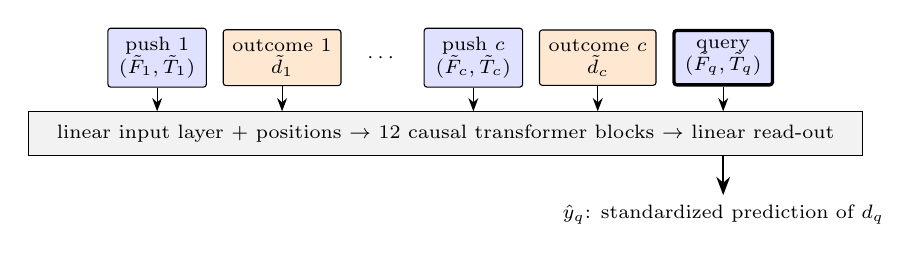
\begin{tikzpicture}[font=\scriptsize, tok/.style={draw, rounded corners=1pt, minimum width=1.25cm, minimum height=0.55cm, align=center}, push/.style={tok, fill=blue!12}, obs/.style={tok, fill=orange!18}]
\node[push] (p1) {push 1\\$(\tilde F_1,\tilde T_1)$};
\node[obs, right=2mm of p1] (o1) {outcome 1\\$\tilde d_1$};
\node[right=2mm of o1] (dots) {$\cdots$};
\node[push, right=2mm of dots] (pc) {push $c$\\$(\tilde F_c,\tilde T_c)$};
\node[obs, right=2mm of pc] (oc) {outcome $c$\\$\tilde d_c$};
\node[push, right=2mm of oc, very thick] (pq) {query\\$(\tilde F_q,\tilde T_q)$};
\node[draw, fill=gray!10, minimum width=10.6cm, minimum height=0.55cm, below=5mm of dots, xshift=8mm] (tf) {linear input layer + positions $\rightarrow$ 12 causal transformer blocks $\rightarrow$ linear read-out};
\foreach \n in {p1,o1,pc,oc,pq} \draw[-{Stealth}] (\n.south) -- (\n.south |- tf.north);
\node[below=5mm of pq.south |- tf.south] (yh) {$\hat y_q$: standardized prediction of $d_q$};
\draw[-{Stealth}, thick] (pq.south |- tf.south) -- (yh.north);
\end{tikzpicture}
\caption{Token layout at test time. Push and outcome tokens alternate. The prediction for a push is read at that push's token; causal attention means it depends on the $c$ earlier push--outcome pairs and the query push, never on the query outcome.}
\label{fig:tokens}
\end{figure}

Each token is a 5-vector: a push is $[\tilde F,\tilde T,0,0,0]$ and an outcome is $[0,0,\tilde d,\widetilde{\mathrm{asinh}}(d/0.01),1]$. A tilde means standardized with training mean and standard deviation, the second outcome feature standardizes $\mathrm{asinh}(d/0.01\,\mathrm{m})$ to compress large displacements, and the final 1 marks outcome tokens. A learned linear layer maps tokens to 256 dimensions and learned position embeddings are added. The network has 12 pre-layer-norm blocks with 8-head causal self-attention and a $4\times$ GELU feed-forward layer, a final layer norm and a linear output: 9,485,057 parameters, no dropout. This follows the GPT-2-family~\cite{radford2019} size used by Garg et al.\ (12 layers, 8 heads, width 256)~\cite{garg2022,vaswani2017}, written from scratch in PyTorch.

A training row is 11 distinct pushes from one cube in random order (22 tokens). With $y_{nj}$ the standardized clean displacement of push $j$ in row $n$, and $\hat y_{nj}=f_\theta(\text{tokens up to push token }j)$, we minimize over batches of $N=256$ rows
\begin{equation}
\mathcal L(\theta)=\frac{1}{11N}\sum_{n=1}^{N}\sum_{j=1}^{11}\big(\hat y_{nj}-y_{nj}\big)^2 .
\end{equation}
Position $j$ has $j-1$ context pushes, so one model is trained for every context length from 0 to 10. We use AdamW~\cite{loshchilov2017} for 150,000 steps with linear warm-up and cosine decay, and keep the checkpoint with the lowest validation loss. Table~\ref{tab:hp} (Appendix~\ref{app:hp}) lists every hyperparameter with how it was chosen. No hyperparameter was tuned by search. In particular, we kept Garg et al.'s learning rate $10^{-4}$ but not their optimizer (Adam), batch size (64), step count (500k) or curriculum.

\subsection{Reference estimators}\label{sec:refs}
\textbf{Bayes (training prior)} is the main reference. Its parameter is $\theta=(m,\mu)$ with the training prior $p(\theta)$. Let context observations be grouped by identical action $a_g$, with mean outcome $\bar d_g$ over $n_g$ distinct measurements (exact copies are removed first), and let $f(\theta,a)$ be Eq.~\eqref{eq:law}, clipped at zero. It predicts the posterior mean
\begin{equation}
\hat d_q=\frac{\int f(\theta,a_q)\,p(\theta)\prod_g\mathcal N\!\big(\bar d_g;f(\theta,a_g),\,\sigma_d^2/n_g+\tau^2(\theta,a_g)\big)d\theta}{\int p(\theta)\prod_g\mathcal N\!\big(\bar d_g;f(\theta,a_g),\,\sigma_d^2/n_g+\tau^2(\theta,a_g)\big)d\theta},
\label{eq:bayes}
\end{equation}
with measurement noise $\sigma_d=0$ here. The small term $\tau=9.5\times10^{-7}f+10^{-4}$ m allows for numerical mismatch between simulator and formula. The integral uses adaptive nested quadrature because the posterior is very narrow (Appendix~\ref{app:bayes}). Because of $\tau$, this is optimal for a slightly softened likelihood, so at very small errors it is not a strict lower bound. A \textbf{broad-prior Bayes} ($m\sim$ log-uniform$[0.35,2.0]$, $\mu\sim$ uniform$[0.2,0.7]$) is used for heavy cubes. A \textbf{physics fit} uses the context alone. If it contains pushes at the query force, it fits $d=hT^2$ to them, $h=\sum_i d_iT_i^2/\sum_i T_i^4$, and predicts $hT_q^2$. Otherwise, if two moving pushes have forces at least 3 N apart, it fits $(A,B)$ in Eq.~\eqref{eq:law} by least squares. Otherwise it reports \emph{not determined}. The \textbf{no-context} baseline is each method at $c=0$. The \textbf{oracle} (true $m,\mu$) reproduces the target exactly.

\subsection{Experiments, metrics and controls}\label{sec:exps}
All experiments evaluate the same frozen checkpoint. Each compares conditions on the same cubes and, within an experiment's paired cells, the same query.

\textbf{E1, amount of context} (100 cubes): each cube has one ordered list of 10 random context pushes and one random query; $c\in\{0,1,2,4,8,10\}$ uses the first $c$.

\textbf{E2, force diversity} (50 cubes): the query force is drawn from $[17,22]$ N. Four context types are crossed (Table~\ref{tab:e2design}). For a given cube and $c$, all four use the same set of durations (none equal to the query's), and context order is randomized. Force diversity is therefore the intended difference between same-force and distinct-force cells.
\begin{table}[t]
\centering\footnotesize
\caption{E2 context cells. ``New'' means all context forces are at least 3 N from the query force $F_q$.}
\label{tab:e2design}
\setlength{\tabcolsep}{3pt}
\begin{tabular}{lll}
\toprule
 & Context all at one force & Context at distinct forces\\
\midrule
Familiar-force query & A: all at $F_q$ ($c=1,2,4$) & C: includes $F_q$; others $\ge1$ N away ($c=2,4$)\\
New-force query & B: one force $\ge3$ N from $F_q$ ($c=2,4$) & D: all $\ge3$ N from $F_q$ ($c=2,4$)\\
\bottomrule
\end{tabular}
\end{table}

\textbf{E3, redundancy} (50 cubes): two base pushes whose forces bracket a new-force query (each at least 3 N away) are followed by $k\in\{0,1,2,4\}$ exact copies of them. Without noise, a copy and a fresh repeat have identical numbers, so this tests only robustness to duplication, \emph{not} the value of repeated noisy measurements.

\textbf{E4, out of range} (50 cubes): as E1, with $m\sim$ log-uniform$[1.5,2.0]$ kg, $c\in\{0,2,10\}$, no retraining.

\textbf{Metrics.} We report standardized MSE, the squared error against the clean displacement divided by the training variance of $d$ ($2.33$ m$^2$, the same denominator for every method), and median relative error $|\hat d-d|/d$. The proposal's NMSE$(c)=$MSE$(c)/$MSE$(0)$ would use a different denominator for each method, so we use a shared one. \textbf{Uncertainty:} error bars are $\pm1$ standard error of the squared error across test cubes. For paired contrasts we give the mean per-cube difference in squared error with a 95\% bootstrap interval (2,000 resamples of cubes). We pair by cube because cube-to-cube difficulty varies widely and cancels in the difference. Both describe variation over \emph{test cubes for one trained model}, which is the right measure for asking whether a gap for \emph{this} model would persist on new cubes. They do not include training-seed variation, which we have not measured.

\textbf{Controls and remaining confounds.} Cubes are disjoint across splits, actions are independent of the hidden parameters, and all methods score the same items. E1 uses nested prefixes. However: (i) training contexts use random forces, so E2's single-force contexts are themselves a shift from training, and a same-versus-distinct gap in the transformer could partly reflect familiarity rather than information; (ii) the transformer and Bayes do not receive equal advantages, since Bayes is given the law and prior; it is a bound on what the context supports, not a competitor trained with equal resources; (iii) in E4 the force and duration ranges are unchanged, but heavier cubes slide shorter distances, which changes the scale of both inputs and errors; (iv) E3 changes length and duplication together, because there is no control that appends equally uninformative \emph{fresh} pushes.

\section{Results}
All numbers below come from the pilot run of Nov.\ 16 (seed 0, checkpoint at step 118,000) and its saved result tables.

\subsection{Training}
\begin{figure}[t]
\centering
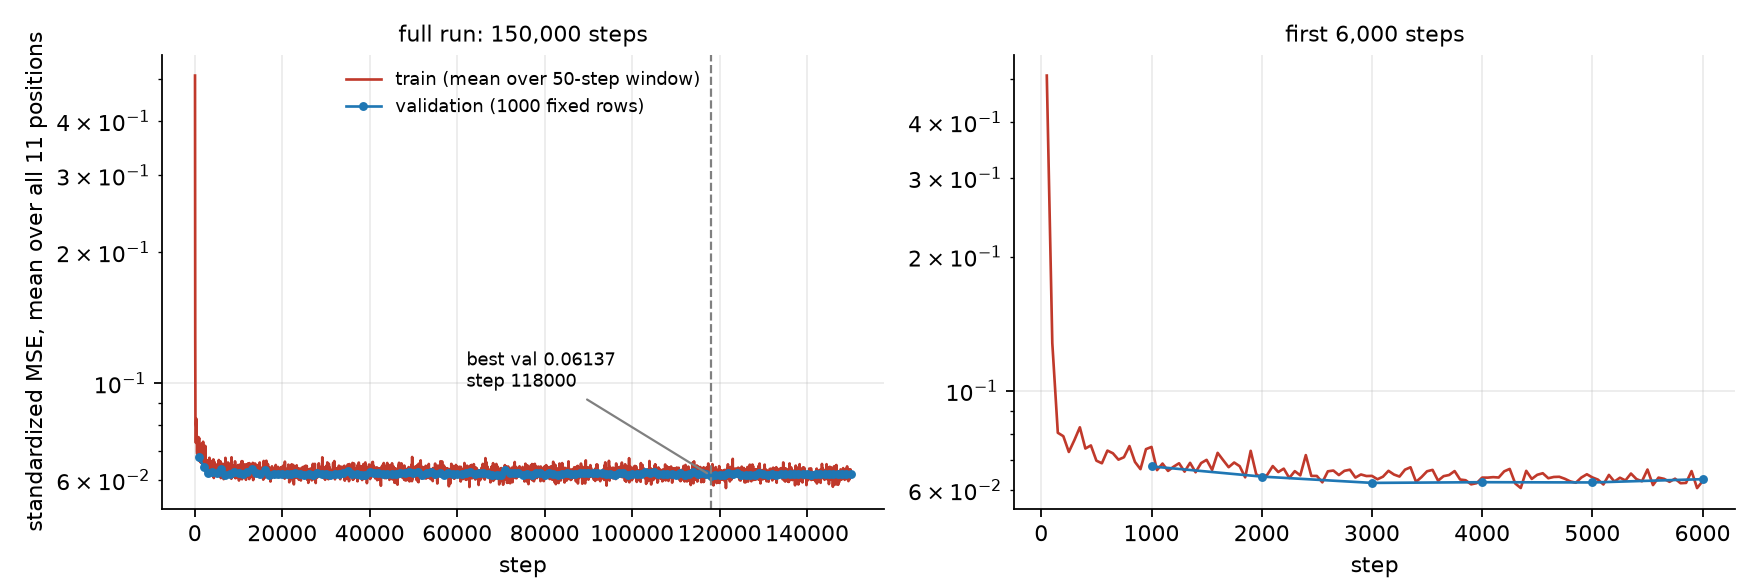
\includegraphics[width=\linewidth]{figures/fig_training.png}
\caption{Training loss (mean over 50-step windows) and validation loss (every 1,000 steps), standardized MSE over all 11 positions, logarithmic $y$-axis so that late changes stay visible. Left: full run; right: first 6,000 steps. One seed, so no error band. The plateau near $0.06$ is almost entirely the no-context position.}
\label{fig:train}
\end{figure}
\begin{figure}[t]
\centering
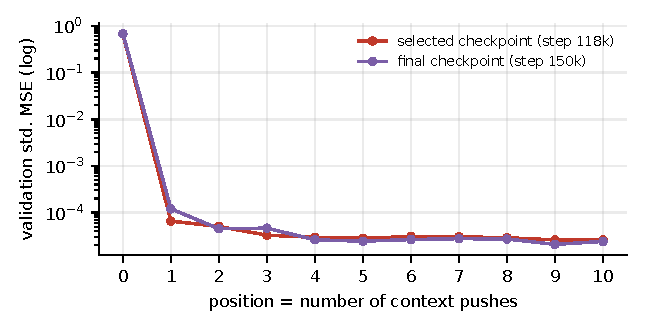
\includegraphics[width=0.62\linewidth]{figures/fig_per_position.pdf}
\caption{Validation standardized MSE at each of the 11 prediction positions for the selected and final checkpoints, on 1,000 fixed validation sequences. Logarithmic axis: position 0 is four orders of magnitude above the rest.}
\label{fig:perpos}
\end{figure}
Training and validation loss track each other (Figure~\ref{fig:train}), and training was stable. The curves hide an important fact (Figure~\ref{fig:perpos}). At position 0, with no context, no method can identify the cube, and its error (0.675) makes up 99.95\% of the average loss. At positions 1--10 the error is between $2.6\times10^{-5}$ and $6.6\times10^{-5}$. So selecting the checkpoint by average validation loss selects mostly on no-context error. The best checkpoint (loss 0.0614, step 118,000) and the final one (0.0619) differ little in aggregate but, as Section~\ref{sec:e2} shows, can differ on the contrast we care about.

\subsection{E1: context helps, then the transformer plateaus}
\begin{figure}[t]
\centering
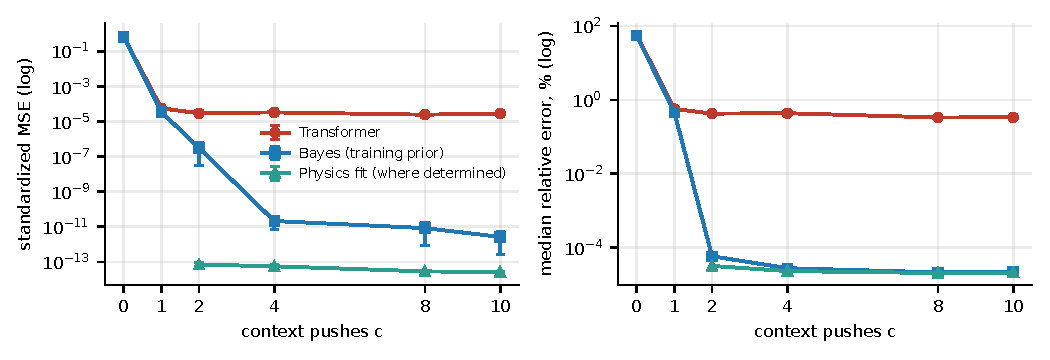
\includegraphics[width=\linewidth]{figures/fig_e1.pdf}
\caption{E1 on 100 unseen cubes. Left: standardized MSE ($\pm1$ SE over cubes; lower bars are clipped where the SE is comparable to the mean). Right: median relative error. Logarithmic $y$-axes are needed because methods differ by up to eleven orders of magnitude. The physics fit is plotted only where determined (56/100 cubes at $c=2$, 99/100 at $c=4$, all at $c\ge8$), so its points are not over the same cubes as the others.}
\label{fig:e1}
\end{figure}
\begin{table}[t]
\centering\small
\caption{E1 median relative error (\%). Same 100 cubes at every $c$.}
\label{tab:e1}
\begin{tabular}{lcccccc}
\toprule
Context size $c$ & 0 & 1 & 2 & 4 & 8 & 10\\
\midrule
Transformer & 56.3 & 0.570 & 0.426 & 0.437 & 0.334 & 0.338\\
Bayes, training prior & 55.2 & 0.458 & $5.8\times10^{-5}$ & $2.8\times10^{-5}$ & $2.1\times10^{-5}$ & $2.2\times10^{-5}$\\
\bottomrule
\end{tabular}
\end{table}
At $c=0$ the transformer's MSE is statistically indistinguishable from Bayes' (paired difference $-0.028$ m$^2$, 95\% interval $[-0.127, 0.059]$): it has learned roughly the prior-average prediction. A single push lowers median error from 56.3\% to 0.57\% (Table~\ref{tab:e1}, Figure~\ref{fig:e1}), so the model clearly uses its context. From $c=2$ the transformer shows no clear further improvement (standardized MSE between $2.4$ and $3.3\times10^{-5}$), while Bayes improves from $3.1\times10^{-7}$ at $c=2$ to $2.1\times10^{-11}$ or below from $c=4$ on. A 0.43\% error is accurate in practical terms, but it is far from what the two observations permit: \textbf{H1 is not supported}, since the second observation does not bring the transformer close to the optimal estimator. We do not yet know what causes the plateau. Candidates are the loss weighting above, only 1,000 training cubes, optimization or numerical precision limits; none has been tested.

\subsection{Why one push already works}\label{sec:onepush}
A 0.57\% error after one observation looks suspicious, because one equation cannot fix two unknowns. The explanation is the prior. One push restricts $(A,B)$ to a line, and the bounded ranges cut that line to a short segment along which predictions at other forces barely change. For example, cubes $(m,\mu)=(1.0, 0.450)$ and $(1.2, 0.3244)$ give the same 0.794 m for a 20 N, 150 ms push, yet their predictions at 24 N differ by only 0.75\%. Exact Bayes at $c=1$ reaches 0.458\% median error, so the transformer's MSE ($1.31\times10^{-4}$ m$^2$) is about 1.6 times that of the best achievable ($8.2\times10^{-5}$ m$^2$). We also audited the pipeline for leakage. Writing the true query outcome into the query's outcome slot changes the prediction by exactly zero; swapping in another cube's context raises median error to 71\%; and scaling the observed $d_1$ by 1.01 scales the prediction almost as exact Bayes does (elasticity 0.995 vs.\ 1.001). These checks found no leak. The practical consequence is that this prior makes one push very informative, which leaves little room for later pushes to matter at the transformer's accuracy.

\subsection{E2: does force diversity matter?}\label{sec:e2}
\begin{figure}[t]
\centering
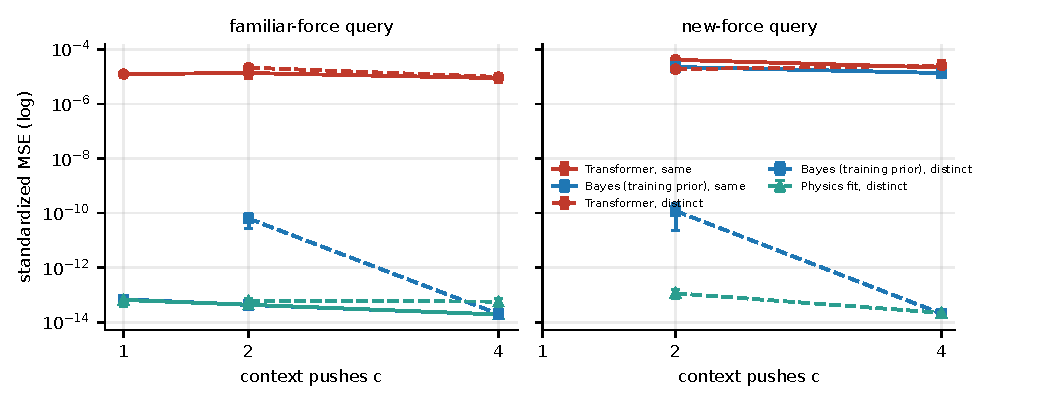
\includegraphics[width=\linewidth]{figures/fig_e2.pdf}
\caption{E2 on 50 cubes: standardized MSE ($\pm1$ SE over cubes, log $y$-axis). Solid lines: same-force contexts (cells A, B); dashed: distinct-force contexts (C, D). Left: familiar-force query; right: new-force query.}
\label{fig:e2}
\end{figure}
\begin{table}[t]
\centering\small
\caption{E2 new-force query: paired difference in squared error, same-force minus distinct-force (cell B $-$ cell D), in $10^{-5}$ m$^2$ with 95\% bootstrap intervals over 50 cubes. Positive means diversity helped.}
\label{tab:e2}
\begin{tabular}{lcc}
\toprule
 & $c=2$ & $c=4$\\
\midrule
Bayes, training prior & $+5.25$ $[2.49, 8.49]$ & $+3.15$ $[1.93, 4.59]$\\
Transformer, selected checkpoint (step 118k) & $+5.22$ $[1.52, 10.2]$ & $-0.93$ $[-6.62, 2.81]$\\
Transformer, final checkpoint (150k, sensitivity) & $+4.36$ $[0.38, 9.41]$ & $+3.00$ $[0.47, 6.24]$\\
\bottomrule
\end{tabular}
\end{table}
The reference behaves as the physics predicts (Figure~\ref{fig:e2}, right). With a new-force query, same-force contexts leave Bayes at a standardized MSE of $2.2$ and $1.3\times10^{-5}$ ($c=2,4$), while distinct forces take it to $1.2\times10^{-10}$ and below. So the design does create two equal-length contexts with different information. For the transformer, diversity helps at $c=2$ by about as much as it helps Bayes in absolute squared error (Table~\ref{tab:e2}). At $c=4$ the selected checkpoint shows no benefit, but the final checkpoint of the \emph{same run} shows one with an interval excluding zero. We therefore call E2 at $c=4$ \textbf{inconclusive}. In every case the transformer's error with distinct forces (1 to $3\times10^{-5}$) stays many orders of magnitude above Bayes', so it does not exploit diversity as an exact reasoner could. With a familiar-force query (left panel) we see no reliable difference between the two context types for the transformer; the difference there at $c=2$ ($-1.8\times10^{-5}$ m$^2$, interval including zero) is about a third of the size of the new-force effect, a reminder of how noisy contrasts at this scale are.

The scale matters for interpreting \textbf{H2}. The information effect, as measured by what same-force Bayes cannot recover ($\sim\!10^{-5}$), is about as large as the transformer's own error floor. Noise-free data with this prior is therefore a weak test of H2 for a model at this accuracy.

\subsection{E3: duplicated observations (noise-free)}
\begin{figure}[t]
\centering
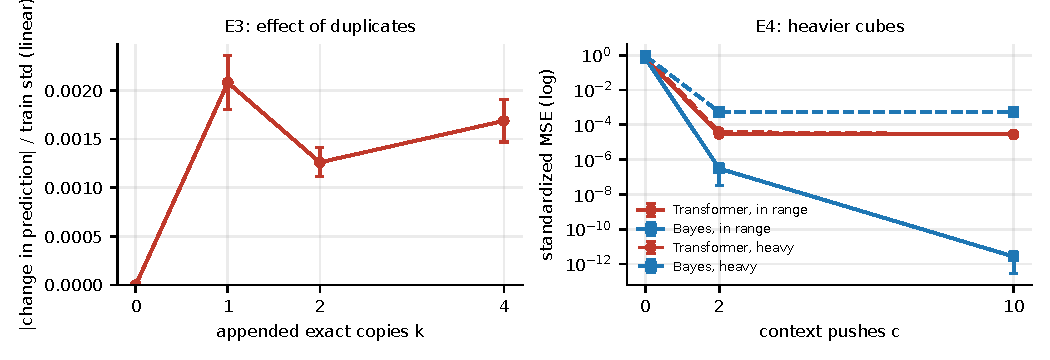
\includegraphics[width=\linewidth]{figures/fig_e3_e4.pdf}
\caption{Left: E3, mean absolute change of the prediction relative to $k=0$ after appending $k$ exact copies, divided by the training standard deviation of $d$ ($\pm1$ SE over 50 cubes). Bayes and the physics fit change by exactly zero because they remove copies (not drawable on a log axis, so the axis is linear). Right: E4, standardized MSE in and out of the training mass range (log axis).}
\label{fig:e3e4}
\end{figure}
Appending copies moves the transformer's prediction by 3.2, 1.9 and 2.6 mm on average for $k=1,2,4$ (largest 11 mm), whereas references do not move (Figure~\ref{fig:e3e4}, left). Its error stays between $2.2$ and $2.7\times10^{-5}$, within one standard error. Duplication perturbs the prediction slightly without a detectable systematic cost. This covers only the noise-free half of \textbf{H3}.

\subsection{E4: heavier cubes than in training}
\begin{table}[t]
\centering\small
\caption{Median relative error (\%) for in-range (100 cubes) and heavy (50 cubes) tests.}
\label{tab:e4}
\begin{tabular}{llccc}
\toprule
Set & $c$ & Transformer & Bayes (training prior) & Bayes (broad prior)\\
\midrule
In range & 2 & 0.43 & $5.8\times10^{-5}$ & $5.3\times10^{-5}$\\
In range & 10 & 0.34 & $2.2\times10^{-5}$ & $2.1\times10^{-5}$\\
Heavy & 0 & 544 & 543 & 933\\
Heavy & 2 & 2.36 & 1.99 & $3.9\times10^{-4}$\\
Heavy & 10 & 2.27 & 1.56 & $8\times10^{-5}$\\
\bottomrule
\end{tabular}
\end{table}
On heavy cubes the transformer still gains from context (544\% to 2.3\%, Table~\ref{tab:e4}), but at $c=10$ its median relative error is about seven times its in-range value. Two readings need care. First, standardized MSE looks the same in and out of range (Figure~\ref{fig:e3e4}, right) only because heavy cubes slide shorter distances; relative error shows the degradation. Second, the transformer beats training-prior Bayes in MSE on heavy cubes, but that estimator cannot represent $m>1.5$ kg; in median relative error the transformer is slightly worse than it, and far worse than broad-prior Bayes. E2 and E3 were not repeated out of range, so \textbf{H4} is only partly tested.

\section{Discussion}
\textbf{What we learned.} (1) A small transformer trained from scratch uses push history to adapt to unseen cubes within this idealized dynamics. (2) Most of its gain comes from the first push, and an exact estimator shows that this is largely a property of the prior. (3) The transformer stops improving where the optimal estimator keeps improving by many orders of magnitude. (4) An equal-length contrast in information is clearly present for Bayes, but our current model and noise-free design cannot resolve it reliably for the transformer. (5) Average validation loss is a poor selection signal for context-dependent behavior: here it is almost all no-context error, and two checkpoints from one run disagree on a headline contrast.

\textbf{Limitations.} One training seed; 1,000 training cubes; a short run; no measurement noise; small test sets for E2--E4; idealized 1D dynamics that match the analytic reference by construction; structured test contexts that differ from random training contexts; no hyperparameter search. Nothing here supports claims about real contact, real robots or language models.

\subsection{Work in progress and plan for V2}\label{sec:progress}
\inprog{\textbf{Seeds.} Retrain with at least three seeds and report mean and standard error across seeds, keeping test sets fixed. This decides whether the $c=4$ E2 result and the plateau are stable. The pilot took 0.56 GPU-hours per seed on an RTX 4090.}

\inprog{\textbf{Selection metric.} Select checkpoints on the mean loss over positions 1--10, decided before looking at test results, and report both rules.}

\inprog{\textbf{Plateau diagnosis}, one change at a time against the pilot: (a) reweight positions or predict a log target; (b) ten times more training cubes; (c) longer training; (d) full-precision matrix multiplication. A change that lowers the error at $c\ge2$ identifies a cause.}

\inprog{\textbf{Measurement noise} ($\sigma_d\approx0.048$ m, 5\% of the median training displacement), retraining per noise level. Compare fresh repeats against exact copies at equal length: an information-using predictor should improve with fresh repeats and not with copies. We expect noise to raise Bayes' error toward the transformer's range, making E2 discriminative, but this is untested. The Bayes code has the $\sigma_d$ term, but its predictor fixes $\sigma_d=0$, so it must be exposed and re-validated first.}

\inprog{\textbf{If time permits:} a wider prior so that one push is less decisive; E2 and E3 on heavy cubes; other out-of-range directions.}

\clearpage
\begin{thebibliography}{99}\small
\bibitem{brown2020} T.~B. Brown, B.~Mann, N.~Ryder, M.~Subbiah, et al. Language models are few-shot learners. \emph{arXiv:2005.14165}, 2020.
\bibitem{garg2022} S.~Garg, D.~Tsipras, P.~Liang, and G.~Valiant. What can transformers learn in-context? A case study of simple function classes. \emph{arXiv:2208.01066}, 2022.
\bibitem{akyurek2022} E.~Aky\"urek, D.~Schuurmans, J.~Andreas, T.~Ma, and D.~Zhou. What learning algorithm is in-context learning? Investigations with linear models. \emph{arXiv:2211.15661}, 2022. ICLR 2023.
\bibitem{vonoswald2022} J.~von Oswald, E.~Niklasson, E.~Randazzo, J.~Sacramento, A.~Mordvintsev, A.~Zhmoginov, et al. Transformers learn in-context by gradient descent. \emph{arXiv:2212.07677}, 2022.
\bibitem{ahn2023} K.~Ahn, X.~Cheng, H.~Daneshmand, and S.~Sra. Transformers learn to implement preconditioned gradient descent for in-context learning. \emph{arXiv:2306.00297}, 2023. NeurIPS 2023.
\bibitem{zhang2023} R.~Zhang, S.~Frei, and P.~L. Bartlett. Trained transformers learn linear models in-context. \emph{arXiv:2306.09927}, 2023.
\bibitem{fu2023} D.~Fu, T.-Q. Chen, R.~Jia, and V.~Sharan. Transformers learn to achieve second-order convergence rates for in-context linear regression. \emph{arXiv:2310.17086}, 2023. NeurIPS 2024.
\bibitem{shen2023} L.~Shen, A.~Mishra, and D.~Khashabi. Do pretrained transformers learn in-context by gradient descent? \emph{arXiv:2310.08540}, 2023.
\bibitem{bai2023} Y.~Bai, F.~Chen, H.~Wang, C.~Xiong, and S.~Mei. Transformers as statisticians: Provable in-context learning with in-context algorithm selection. \emph{arXiv:2306.04637}, 2023.
\bibitem{li2023} Y.~Li, M.~E. Ildiz, D.~Papailiopoulos, and S.~Oymak. Transformers as algorithms: Generalization and stability in in-context learning. \emph{arXiv:2301.07067}, 2023.
\bibitem{wang2025} K.~A. Wang, J.~Shi, and E.~B. Fox. Test-time regression: A unifying framework for designing sequence models with associative memory. \emph{arXiv:2501.12352}, 2025.
\bibitem{xie2021} S.~M. Xie, A.~Raghunathan, P.~Liang, and T.~Ma. An explanation of in-context learning as implicit Bayesian inference. \emph{arXiv:2111.02080}, 2021. ICLR 2022.
\bibitem{muller2021} S.~M\"uller, N.~Hollmann, S.~Pineda Arango, J.~Grabocka, and F.~Hutter. Transformers can do Bayesian inference. \emph{arXiv:2112.10510}, 2021. ICLR 2022.
\bibitem{panwar2023} M.~Panwar, K.~Ahuja, and N.~Goyal. In-context learning through the Bayesian prism. \emph{arXiv:2306.04891}, 2023. ICLR 2024.
\bibitem{chan2022} S.~C.~Y. Chan, A.~Santoro, A.~K. Lampinen, J.~X. Wang, A.~Singh, P.~H. Richemond, et al. Data distributional properties drive emergent in-context learning in transformers. \emph{arXiv:2205.05055}, 2022. NeurIPS 2022.
\bibitem{singh2023} A.~K. Singh, S.~C.~Y. Chan, T.~Moskovitz, E.~Grant, A.~M. Saxe, and F.~Hill. The transient nature of emergent in-context learning in transformers. \emph{arXiv:2311.08360}, 2023.
\bibitem{olsson2022} C.~Olsson, N.~Elhage, N.~Nanda, N.~Joseph, N.~DasSarma, T.~Henighan, et al. In-context learning and induction heads. \emph{arXiv:2209.11895}, 2022.
\bibitem{raventos2023} A.~Ravent\'os, M.~Paul, F.~Chen, and S.~Ganguli. Pretraining task diversity and the emergence of non-Bayesian in-context learning for regression. \emph{arXiv:2306.15063}, 2023.
\bibitem{forgione2023} M.~Forgione, F.~Pura, and D.~Piga. From system models to class models: An in-context learning paradigm. \emph{arXiv:2308.13380}, 2023.
\bibitem{bazzi2024} M.~Bianchi Bazzi, A.~A. Shahid, C.~Agia, J.~Alora, M.~Forgione, D.~Piga, et al. RoboMorph: In-context meta-learning for robot dynamics modeling. \emph{arXiv:2409.11815}, 2024.
\bibitem{zhang2024} X.~Zhang, S.~Liu, P.~Huang, W.~J. Han, Y.~Lyu, M.~Xu, et al. Dynamics as prompts: In-context learning for sim-to-real system identifications. \emph{arXiv:2410.20357}, 2024.
\bibitem{mason1986} M.~T. Mason. Mechanics and planning of manipulator pushing operations. \emph{International Journal of Robotics Research}, 5(3):53--71, 1986.
\bibitem{yu2016} K.-T. Yu, M.~Bauza, N.~Fazeli, and A.~Rodriguez. More than a million ways to be pushed: A high-fidelity experimental dataset of planar pushing. \emph{arXiv:1604.04038}, 2016. IROS 2016.
\bibitem{song2020} C.~Song and A.~Boularias. Learning to slide unknown objects with differentiable physics simulations. \emph{arXiv:2005.05456}, 2020. RSS 2020.
\bibitem{xu2019} Z.~Xu, J.~Wu, A.~Zeng, J.~B. Tenenbaum, and S.~Song. DensePhysNet: Learning dense physical object representations via multi-step dynamic interactions. \emph{arXiv:1906.03853}, 2019. RSS 2019.
\bibitem{yu2017} W.~Yu, J.~Tan, C.~K. Liu, and G.~Turk. Preparing for the unknown: Learning a universal policy with online system identification. \emph{arXiv:1702.02453}, 2017. RSS 2017.
\bibitem{kumar2021} A.~Kumar, Z.~Fu, D.~Pathak, and J.~Malik. RMA: Rapid motor adaptation for legged robots. \emph{arXiv:2107.04034}, 2021. RSS 2021.
\bibitem{lee2020} K.~Lee, Y.~Seo, S.~Lee, H.~Lee, and J.~Shin. Context-aware dynamics model for generalization in model-based reinforcement learning. \emph{arXiv:2005.06800}, 2020. ICML 2020.
\bibitem{nagabandi2018} A.~Nagabandi, I.~Clavera, S.~Liu, R.~S. Fearing, P.~Abbeel, S.~Levine, et al. Learning to adapt in dynamic, real-world environments through meta-reinforcement learning. \emph{arXiv:1803.11347}, 2018.
\bibitem{peng2017} X.~B. Peng, M.~Andrychowicz, W.~Zaremba, and P.~Abbeel. Sim-to-real transfer of robotic control with dynamics randomization. \emph{arXiv:1710.06537}, 2017.
\bibitem{lindley1956} D.~V. Lindley. On a measure of the information provided by an experiment. \emph{Annals of Mathematical Statistics}, 27(4):986--1005, 1956.
\bibitem{chaloner1995} K.~Chaloner and I.~Verdinelli. Bayesian experimental design: A review. \emph{Statistical Science}, 10(3):273--304, 1995.
\bibitem{achterhold2021} J.~Achterhold and J.~St\"uckler. Explore the context: Optimal data collection for context-conditional dynamics models. \emph{arXiv:2102.11394}, 2021. AISTATS 2021.
\bibitem{todorov2012} E.~Todorov, T.~Erez, and Y.~Tassa. MuJoCo: A physics engine for model-based control. In \emph{IEEE/RSJ International Conference on Intelligent Robots and Systems}, pages 5026--5033, 2012.
\bibitem{radford2019} A.~Radford, J.~Wu, R.~Child, D.~Luan, D.~Amodei, and I.~Sutskever. Language models are unsupervised multitask learners. OpenAI technical report, 2019.
\bibitem{vaswani2017} A.~Vaswani, N.~Shazeer, N.~Parmar, J.~Uszkoreit, L.~Jones, A.~N. Gomez, et al. Attention is all you need. \emph{arXiv:1706.03762}, 2017. NeurIPS 2017.
\bibitem{loshchilov2017} I.~Loshchilov and F.~Hutter. Decoupled weight decay regularization. \emph{arXiv:1711.05101}, 2017. ICLR 2019.
\end{thebibliography}

\clearpage
\appendix
\section{Hyperparameters and how they were chosen}\label{app:hp}
No value was selected by a hyperparameter search. ``Pilot choice'' means it was fixed in the pilot specification before training, without a supporting experiment; those are the weakest choices and candidates for ablation.
\begin{table}[ht]
\centering\small
\caption{All model, training and data settings of the pilot run.}
\label{tab:hp}
\begin{tabular}{>{\raggedright}p{3.2cm}>{\raggedright}p{3.0cm}p{6.4cm}}
\toprule
Setting & Value & Basis\\
\midrule
Layers / width / heads & 12 / 256 / 8 & Garg et al.~\cite{garg2022}: a size shown to learn several function classes in context.\\
Feed-forward, activation & 1024, GELU & GPT-2 convention ($4\times$ width)~\cite{radford2019}.\\
Dropout & 0 & Pilot choice; every row is a freshly sampled sub-sequence.\\
Weight initialization & $\mathcal N(0,0.02^2)$, zero bias & GPT-2 convention.\\
Sequence length & 22 tokens & 10 context pushes plus a query, as the experiments require.\\
Optimizer & AdamW~\cite{loshchilov2017}, $\beta=(0.9,0.999)$, $\epsilon=10^{-8}$ & Pilot choice (Garg et al.\ use Adam); PyTorch default $\beta,\epsilon$.\\
Learning rate & $10^{-4}$ & Garg et al.~\cite{garg2022}, who use it for all their function classes.\\
Weight decay & 0.01 & Pilot choice; applied to all parameters.\\
Batch size & 256 & Pilot choice (Garg et al.\ use 64).\\
Gradient clipping & global norm 1.0 & Pilot choice, for stability.\\
Warm-up & 2,000 steps & 5\% of steps, capped at 2,000; pilot choice.\\
Schedule & cosine to 0 & Pilot choice.\\
Training steps & 150,000 & Set from a throughput benchmark to fit a 30--45 minute budget. This exceeds a 100k limit in our earlier internal protocol.\\
Precision & float32; TF32 matmul allowed & Speed; untested as a cause of the plateau.\\
Validation / selection & every 1,000 steps; lowest loss & Pilot choice; Section~4.1 shows its weakness.\\
$m$, $\mu$ prior & log-uniform [0.5,1.5]; uniform [0.3,0.6] & Chosen so all in-range pushes move the cube; Section~\ref{sec:onepush} shows the cost.\\
$F$, $k$ ranges & [13,26] N; 100--200 ms & Pilot choice; $\min F$ exceeds the largest friction force.\\
Training data & 1,000 cubes $\times$ 32 pushes & Pilot budget (proposal planned about 10,000 cubes).\\
Seed & 0 & Single pilot run.\\
\bottomrule
\end{tabular}
\end{table}

Training-set standardization constants (mean, standard deviation): $F$: 19.48, 3.747 N; $T$: 0.1497, 0.02921 s; $d$: 1.481, 1.528 m; $\mathrm{asinh}(d/0.01\,\mathrm m)$: 5.242, 0.9772.

\section{Why we replaced the contact simulator}\label{app:contact}
The first scene was a free cube (six degrees of freedom) on a plane with MuJoCo box--floor contact. It did not behave like a sliding block. In 1,000 random training-range pushes, 906 rotated more than $1^\circ$ and 105 more than $45^\circ$. In four diagnostic cases the contact was repeatedly lost during the push, and the normal force reached $8$--$41$ times $mg$. While in contact, friction equaled $\mu$ times the normal force, but the normal force was not $mg$. In the worst case the cube left the floor and the displacement was 31.6\% from Eq.~\eqref{eq:law}. The hopping also appeared with no applied force and an initial velocity. About 30 contact and solver settings and several constrained scenes did not give both flat sliding and Coulomb friction. One variant agreed with the formula only because contact chatter averaged out, so we rejected it, and MuJoCo's joint friction-loss option let the cube creep below the friction threshold. We do not claim that MuJoCo is wrong: only that these configurations did not realize our assumptions. We have not established the mechanism.

\section{Bayes computation and checks}\label{app:bayes}
With $u=\log m$, the prior is uniform on a box in $(u,\mu)$. After two distinct forces the posterior's relative width is about $10^{-5}$--$10^{-4}$, much narrower than a cell of a plain $400\times400$ grid. The inner integral over $\mu$ uses the fact that $f$ is affine in $1/\mu$ for a moving push, placing 400 nodes on the window that carries the mass. The outer integral over $u$ uses composite 4-point Gauss--Legendre panels that are subdivided where the log-evidence changes quickly. All sums are computed in log space. On 24 hard cases, doubling the resolution and an independent brute-force implementation agreed to $1.4\times10^{-8}$ and $2.0\times10^{-7}$ relative. An independent implementation matched on 80 real test cases with median relative difference $2\times10^{-15}$. A separate review of synthetic adversarial cases had completed 19 of 23 when it was written up.

\section{Additional tables}
\begin{table}[ht]
\centering\small
\caption{Standardized MSE for E1 (100 cubes). Physics fit omitted because it is defined on different subsets.}
\begin{tabular}{lcccccc}
\toprule
$c$ & 0 & 1 & 2 & 4 & 8 & 10\\
\midrule
Transformer & 0.642 & $5.6\mathrm e{-5}$ & $3.0\mathrm e{-5}$ & $3.3\mathrm e{-5}$ & $2.4\mathrm e{-5}$ & $2.9\mathrm e{-5}$\\
Bayes & 0.654 & $3.5\mathrm e{-5}$ & $3.1\mathrm e{-7}$ & $2.1\mathrm e{-11}$ & $8.4\mathrm e{-12}$ & $2.7\mathrm e{-12}$\\
\bottomrule
\end{tabular}
\end{table}
\begin{table}[ht]
\centering\small
\caption{Standardized MSE for E2 (50 cubes), selected checkpoint.}
\begin{tabular}{llcc}
\toprule
Cell & $c$ & Transformer & Bayes\\
\midrule
A same-force, familiar & 1 / 2 / 4 & 1.2 / 1.4 / 0.88 $\times10^{-5}$ & 6.9 / 4.3 / 1.9 $\times10^{-14}$\\
C distinct, familiar & 2 / 4 & 2.1 / 0.97 $\times10^{-5}$ & $6.3\times10^{-11}$ / $2.0\times10^{-14}$\\
B same-force, new & 2 / 4 & 4.1 / 2.1 $\times10^{-5}$ & 2.2 / 1.3 $\times10^{-5}$\\
D distinct, new & 2 / 4 & 1.9 / 2.5 $\times10^{-5}$ & $1.2\times10^{-10}$ / $2.0\times10^{-14}$\\
\bottomrule
\end{tabular}
\end{table}
Using the final instead of the selected checkpoint changes E1 MSE at $c\ge1$ by roughly 1--18\%, in both directions; the heavy-cube median relative error at $c=10$ is 2.1\% and the E3 mean prediction shifts are 3.5, 2.5 and 3.4 mm.

\section{Reproducing the figures and tables}\label{app:repro}
The repository README for \texttt{report/v1} gives the commands. \texttt{scripts/make\_report\_figures.py} regenerates Figures~\ref{fig:perpos}--\ref{fig:e3e4} from the committed result tables in \texttt{results/pilot\_v1/csv}, and \texttt{scripts/make\_report\_tables.py} prints every result table and the quoted result numbers from the same files. As a check on the data pipeline, we regenerated the pilot dataset on a second machine (a laptop, same MuJoCo 4.0.1): the content hashes of all seven data files and the combined dataset hash match the pilot's. Figure~\ref{fig:train} is the plot saved by the pilot run (its footnote cropped); its raw step-by-step log and the two checkpoints are stored on the training machine and are not yet in the repository. \inprog{Release them for V2.} The full pipeline (simulate data, train, evaluate) can be rerun with \texttt{scripts/make\_pilot\_dataset.py}, \texttt{scripts/train.py} and \texttt{scripts/eval\_run.py}. Pilot identifiers: dataset hash \texttt{f722c512...}, training commit \texttt{e6c51af}, evaluation commit \texttt{2f3d53d}, checkpoint SHA-256 \texttt{6101448e...f230}.

\section{Use of generative AI}\label{app:ai}
\textbf{Proposal stage.} David Jo used Gemini Notebook for a broad literature sweep and Claude to start the codebase, ask about hardware capabilities, and review, edit and transcribe the proposal into LaTeX. Soomi Lee used ChatGPT to brainstorm and assess feasibility, search for papers, edit the proposal and move it from Notion into Overleaf.

\textbf{Pilot (code, experiments, analysis).} The simulator, data, model, training, reference, evaluation and figure code were written with Claude Code (Claude Opus 5.5 and Claude Sonnet 5.5, per the commit history), working as multiple agents under human-approved specifications, with separate agent reviews. Those agents also wrote the pilot's summary, guide, audit of the one-push result and fact-check. The agents ran the pipeline's tests; agent review is not the same as human verification.

\textbf{This report.} David Jo used Claude Code (Claude Sonnet 5.5) to draft this V1 text from the proposal and the saved pilot results, search for and check related work against arXiv titles, authors and abstracts (the CAPTURE description also against parts of its full text) and publisher or index records for non-arXiv items, check the training settings quoted from Garg et al.\ against their paper, and write the report's figure script. Literature descriptions are limited to what those sources state; the authors should read each cited paper before the final version.

\end{document}
